\documentclass[a4paper,fontsize=12bp]{extreport}
\usepackage[T2A]{fontenc}
\usepackage[utf8]{inputenc}
\usepackage[english,russian]{babel}
\usepackage[top = 2cm, bottom = 2 cm]{geometry}
\usepackage{cmap}
\usepackage{graphicx}
\usepackage{listings}
\usepackage{color}
\usepackage{amsmath}
\usepackage{pgfplots}
\usepackage{url}
\usepackage{float}
\usepackage{multirow}
\usepackage{indentfirst}
\usepackage[warn]{mathtext} 
\usepackage{wasysym}
\usepackage{scrextend}
\linespread{.976}

\usepackage{titlesec}
\titleformat*{\section}{\LARGE\bfseries}
\titleformat*{\subsection}{\Large\bfseries}
\titleformat*{\subsubsection}{\large\bfseries}
\titleformat*{\paragraph}{\large\bfseries}
\titleformat*{\subparagraph}{\large\bfseries}


\begin{document}

\section*{Задание}

В многофункциональный центр предоставления государственных и муниципальных услуг (МФЦ) приходят клиенты через интервал времени 3 $\pm$ 2 минуты. Каждому клиенту необходимо получить талон на одном из трех терминалов. Каждый терминал выдает талон с интервалом в 5 $\pm$ 2 минуты. Если в очереди к терминалу находится больше 3 человек, клиент уходит. Также с вероятность 20\%  терминал не будет работать из-за технических неполадок, и тогда клиенту будет отказано. Клиенты приходят по равномерному распределению. 

Если клиент выбирает услугу, связанную с заменой паспорта, ему необходимо сначала пройти в кабинет МВД, находящийся в том же отделении МФЦ. Если в очереди в кабинет уже находится 5 человек, то клиент уходит. С вероятностью 30\%  необходимые документы не будут готовы, и тогда клиент получит отказ в кабинете МВД. Проверка документов  клиента происходит за 10 $\pm$ 5 минут. После получения нужной услуги в кабинете МВД клиент получит направление в кабинет 1 или кабинет 2. В кабинетах 1 и 2 время работы с клиентом составляет 6 $\pm$ 3 минуты. С вероятностью 5\% в данных кабинетах могут возникнуть проблемы с документами, и тогда клиенту будет отказано. 

Если клиент выбирает услугу, несвязанную с заменой паспорта, ему выдают талон в кабинет 3 или 4. Время работы с клиентом в данных кабинетах составляет 8 $\pm$ 4 и 20 $\pm$ 10 минут соответственно. Также с вероятностью 10\% клиенту будет отказано в оказаниии услуги в кабинете в случае отсутствия у него необходимых документов. Если в очереди к кабинету  находится больше 10 человек, клиент уходит. 
 
Промоделировать процесс обслуживания различного числа клиентов. Найти количество отказов на каждом из терминалов и в каждом из кабинетов.
	
\section*{Теоретическая часть}
	
На рис. \ref{fig:1} и \ref{fig:2} представлены схемы концептуальной модели МФЦ:


\begin{figure}[H]
    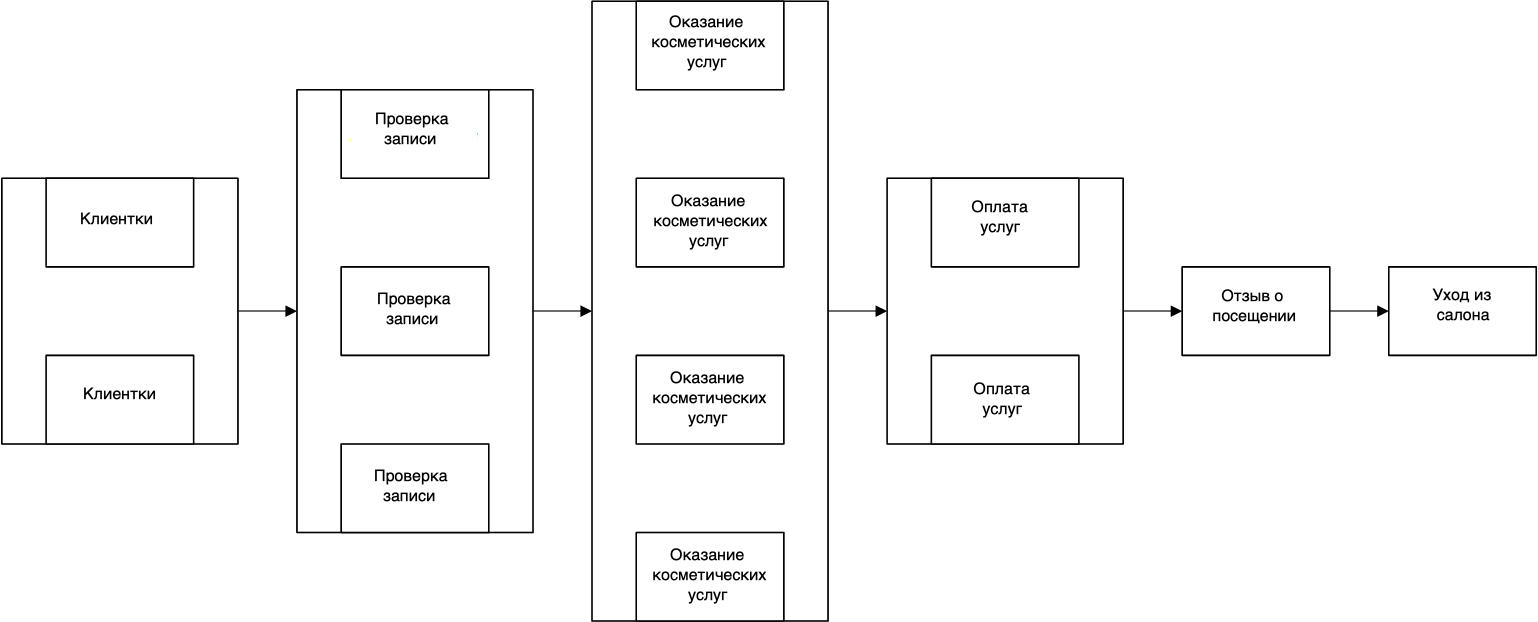
\includegraphics[scale=0.56]{scheme}
    \caption{Структурная схема МФЦ}
    \label{fig:1}
\end{figure}

\begin{figure}[H]
    \includegraphics[scale=0.56]{scheme2}
    \caption{Система массового обслуживания МФЦ}
    \label{fig:2}
\end{figure}

В процессе взаимодействия клиентов с МФЦ возможно: 
\begin{enumerate}
\item режим нормального обслуживания, т.е. клиент выбирает один из свободных терминалов, отдавая предпочтение тому, у которого меньше номер;
\item режим отказа в обслуживании клиента в случае слишком большой очереди или при возникновении проблем с терминалом или документами.\\
\end{enumerate}

При реализации данной работы используется событийный принцип: состояния отдельных устройств изменяются в дискретные моменты времени, совпадающие с моментами времени поступления сообщений в систему, времени поступления окончания задачи, времени поступления аварийных сигналов и т.д.\\
 

\section*{Результаты работы}

100 клиентов: 

\begin{figure}[H]
    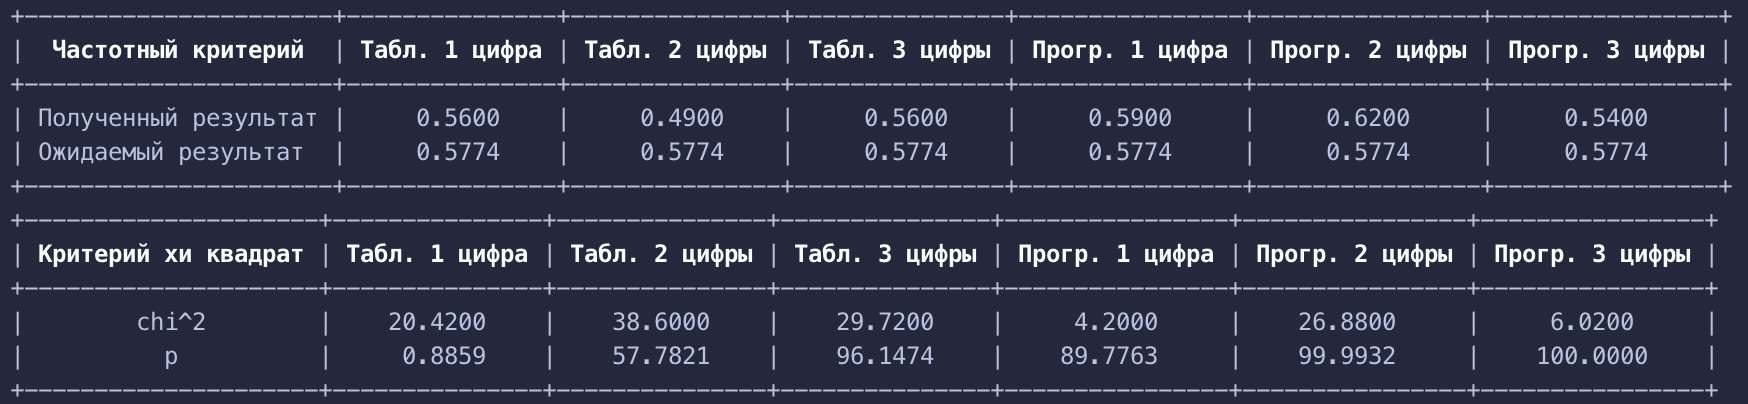
\includegraphics[scale=0.6]{100}
\end{figure}

\newpage
500 клиентов: 

\begin{figure}[H]
    \includegraphics[scale=0.6]{500}
\end{figure}


1000 клиентов: 

\begin{figure}[H]
    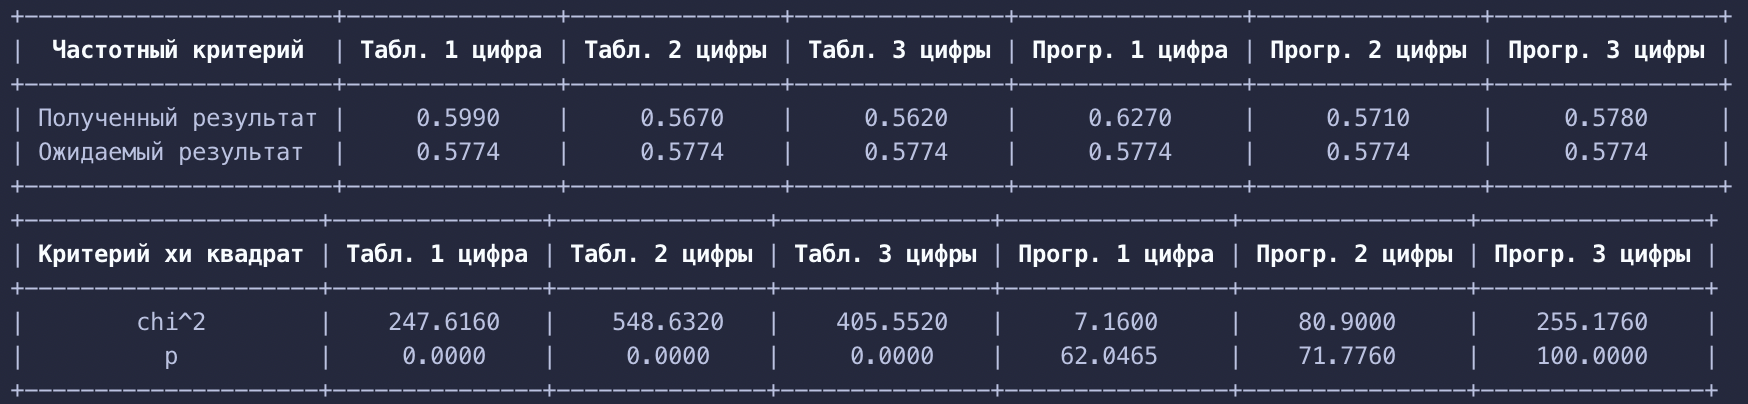
\includegraphics[scale=0.6]{1000}
\end{figure}


10000 клиентов: 

\begin{figure}[H]
    \includegraphics[scale=0.6]{10000}
\end{figure}

Из полученных результатов можно сделать вывод, что меньше всего отказов было получено в кабинетах 1 и 2. Это связано с низким процентом отказов (5\%) и неограниченной длиной очереди. Также мало отказов было в кабинетах 3 и 4, максимальная очередь в которые составляет 10 человек, а вероятность отказа -- 10\%.

Больше всего отказов клиенты получали на терминалах, максимальная длина очереди к которым составляет 3 человека, а вероятность отказа равна 20\%.

\section*{Вывод}
В ходе выполнения лабораторной работы была смоделирована система массового обслуживания МФЦ. При посещении МФЦ клиент проходит через один из трех терминалов, возможно через кабинет МВД и через один из четырех кабинетов. На каждом из этапов клиент может получить отказ в предоставлении услуг.  В ходе моделирования системы было найдено количество отказов на каждом из этапов при разном количестве клиентов.
\end{document}